\chapter{Introduction}
\section{Background}
\par
The modern distribution network has changed more over the last ten years than it has in the previous hundred.
In the past, generation and load were largely separate; power was generated at large stations, and power was consumed by customers after traversing the transmission and distribution networks. 
These days, power is still consumed in the distribution network, but is also generated and manipulated by distributed energy resources (DER). 
\par
DERs are controllable devices in the power network that generate, store, and consume load. 
This includes solar generation (PV), battery storage, and electric vehicles (EV). 
\par
The Tasmanian distribution network is forecast to experience significant increases in these technologies by 2025: \\
\begin{itemize}
	\item 600\% increase in battery storage capacity (from 100MWh to 600MWh) \citep{Jacobs2017}
	\item 170\% increase in PV installation capacity (from 130MW to 220MW) \citep{Jacobs2017}
	\item 39\% of new car sales with be EVs - the highest in the country \citep{AEMO2016}
\end{itemize}

This changing network presents an opportunity to maximize the use of existing assets by delaying the need for network augmentations, while also providing customers with a more reliable supply of power.
However, to achieve this requires sophisticated methods to optimize the power flow to and from the distributed resources \cite{Scott2014}.
\par
One requirement for optimization is an accurate forecast of day-ahead load at the feeder level.
Traditional load forecasting methods do not provide an adequate level of accuracy over a time period this short.
As a result, the optimization of the distributed resources is not as effective as it could be.
\par
To solve this, a neural network-based load forecasting system is proposed.
This system will be applied to Bruny Island, in southern Tasmania, as a case study.
Bruny Island currently has a high penetration of PV and battery technology which is optimized by the Network-aware Coordination (NAC) algorithm \cite{Evan2016}.
Additionally, it is constrained by its feeder during peak holiday periods, necessitating an on-island diesel generator. The load forecasting system will need to be able to perform equally well on holidays, where the load is generally large, and on normal days. 
This makes it a perfect case study to highlight the potential benefits that distributed resources can have in the network.
This project and case study is supported by TasNetworks.

\section{State of the art in load forecasting}
What is clear throughout the literature is that there are a handful, perhaps a dozen or so, of clearly distinct techniques that are commonly applied to load forecasting.
However, these methods are nearly always mixed, matched, and combined to form a complete forecasting system.
As a result, there are a combinatorial number of approaches to forming a load forecasting system.
This section will attempt to cover only the most prolific techniques, and the examples cited will generally also employ techniques which have not been discussed. 
% The reader should not allow this to distract them from focussing on the technique being discussed.

\subsection{Patterns in load profiles}
\label{patterns-profiles}
In a residential setting, such as a residential feeder, power is consumed as a result of customer actions - taking a shower causes the hot water system to consume power to reheat water, turning on a kettle or toaster causes power to be consumed, use of air conditioning results in power consumption, etc.
It is intuitive and reasonable to expect that there would be patterns underlying these actions or behaviours; customers probably take showers more often in the morning, and when it is cold customers are probably more likely to turn on their heaters.
If the feeder in question happens to be in a popular holiday destination, then it might also be the case that overall more power is consumed during holiday periods as a result of more customers being in the area.
Any load forecasting system must be able to intrinsically model these underlying patterns if it is to effectively predict load.
\par
Before looking at load forecasting techniques and systems, we will first delve into the typically available data and investigate what patterns exist.
It needs to be kept in mind though that all conclusions presented here are general; they will likely vary between countries, cultures, and feeders.
Analysis of a specific feeder is undertaken in \hl{section xx}.

\subsubsection{Calendar day}
The most significant factor contributing to a load profile is the calendar day \citep{Weron2006}.
Generally weekdays and weekends have differing load profiles, and even days during the week can be observed to have significantly different profiles.
It can be seen that seasonality normally plays a large role in load variation over a full year, but the extent depends on the location of the feeder.
Different feeders will experience changes in load due to warm and cool weather differently depending on customer behaviour.
Finally, holiday periods cause large deviations from standard profiles and can be difficult to predict due to the relatively few examples available.
Holidays sometimes also affect days adjacent to them, as people may also take these days off work.

\subsubsection{Weather}
Second to calendar day, the most significant factor behind the load profile is the weather \citep{Hippert2001}.
Typically temperature and humidity are considered the most influential, as they drive customers to use heating and cooling which both consume large amounts of power.
More recently, cloud cover and solar irradiance have become increasingly important as they affect rooftop photovoltaic (PV) generation \citet{AEMO2017}.
In regards to PV, it may be further necessary to model its uptake - solar capacity is increasing in Australia \citep{Jacobs2017} and so training data may need to be manipulated to reflect this.

\subsection{Similar day and clustering}
As discussed in section \ref{pattens-profiles}, a load profile is dependent primarily on the calendar day and the weather.
This fact can be used to form a rudimentary load forecasting system by simply finding a load profile from the past that has the most similar calendar day and weather properties to the period being forecast. 
Similarly, a clustering approach can be taken if it is assumed that load profiles will repeat themselves as a result of repeating weather and calendar day patterns.
\par
\citet{Rahman1993} used an expert-system based method to select a set of similar days from the past. 
These days were then modified by use of a lookup table based on differences in temperature and other exogenous factors between the similar and forecast period.
Finally, all similar days were regressed to form a forecast.
\par
\citet{Senjyu1998} used a weighted sum-squared-error between the maximum temperature, minimum temperature, and day type of the period being forecast and previous days to select the most similar five days from the past.
A fuzzy logic system was then used to generate weights to augment the similar days based on differences in weather and differences in load profile between the similar day and the day prior to the forecast day.
This was found to out-perform a more rudimentary systems which only used average load of the similar days.
The load being forecast was approximately 600MW.
\par
\todo[inline]{add some more. Next day load curve forecasting using recurrent neural network structure}


\subsection{Autoregressive integrated moving average}
\todo[inline]{todo Change X to Y for output}
\todo[inline]{todo make consistent with Nomenclature chapter}
Autoregressive integrated moving average (ARIMA) models, introduced by \citet{Box1970}, are used widely for time series forecasting \citep{Weron2006}. 
Generally, ARIMA models are used at the core of the forecasting system, and other methods are used in a supporting role. 
\par
\citet{Bennett2014} used an ARIMAX model to forecast the properties of the next day's load (next day peak demand, next day morning peak, and next day total energy usage). These properties are then provided to a neural network which selects the appropriate cluster for the day, whose load profile mean is then modified to better match the predicted properties.
\\
\citet{Karthika2017} used an ARIMA model to perform a preliminary load forecast, which is then augmented by a support vector machine to account for non-linear exogenous variables such as temperature and day of week.
\par
ARIMA-based models are complex and require a great deal of experience to effectively select appropriate parameters \citep{Desouky2000}.
\par
The ARIMA model is an extension of the autoregressive moving average (ARMA) model, which is comprised of an autoregressive (AR) term and a moving average (MA) term.
\\
Consider a time series $X$, being drawn from some underlying process, with elements $X_{t}, X_{t-1}, ..., X_{0}$. 
\\
An autoregressive model is given by
\begin{equation}
X_{t} = \alpha_{1}X_{t-1} + \alpha_{2}X_{t-2} + \ldots + \alpha_{p}X_{t-p} + \epsilon_{t} = \epsilon_{t} + \sum_{i=1}^{p}\alpha_{i}X_{t-i}
\end{equation}
where $p$ is the order of the AR model, $\alpha$ are the parameters of the model, and $\epsilon_{t}$ is a random normally distributed error with zero mean and variance $\sigma^2$. 
\\ 
A moving average model is given by 
\begin{equation}
X_{t} = \theta_{1}\epsilon_{t-1} + \theta_{2}\epsilon_{t-2} + \ldots + \theta_{q}\epsilon_{t-q} + \epsilon_{t} = \epsilon_{t} + \sum_{i=1}^{q}\theta_{i}\epsilon_{t-i}
\end{equation}
where $q$ is the order of the MA model, $\theta$ are the parameters of the model, and $\epsilon_{t}$ is, again, a random normally distributed error with zero mean and variance $\sigma^2$.
\par
The AR and MA models are combined to form an ARMA model, given by 
\begin{equation}
X_{t} = \epsilon_{t} + \sum_{i=1}^{q}\theta_{i}\epsilon_{t-i} + \sum_{i=1}^{p}\alpha_{i}X_{t-i}
\end{equation}
\par
An ARMA model requires the time series, $X$, being forecast to come from a weakly stationary process.
That is, the mean and autocovariance of the the process do not change with time.
\par
The ARIMA model is an extension to the ARMA model that can be applied when non-stationarity is exhibited by the underlying process.
ARIMA applies differencing to the time series prior to applying the ARMA model to the new time series $\hat{X}$.
This differencing is applied such that $\hat{X}_{t} = X_{t} - X_{t-1}$ and is repeated $d$ times.
Differencing can sometimes be sufficient to make a series stationary, such that it is appropriate for forecasting with an ARMA model.
\par
In order to concisely articulate the ARIMA model, the following notation will be used. The backward shift operator, defined by $\textbf{B}^{m}X_{t} = X_{t-m}$. The difference operator, defined by $\nabla_{s} X_{t} = X_{t} - X_{t-s} = (1 - \textbf{B}^{s})X_{t}$. The parameter functions $\alpha_{p}(\textbf{B}) = 1 - \alpha_{1}\textbf{B} - \ldots - \alpha_{p}\textbf{B}^p$ and $\theta_{q}(\textbf{B}) = 1 + \theta_{1}\textbf{B} + \ldots + \theta_{q}\textbf{B}^q$.
\par
Using this notation, the ARIMA model can be represented as the following
\begin{equation}
\alpha_{p}(\textbf{B})(\nabla_{1}^{d}X_{t}) = \theta_{q}(\textbf{B})\epsilon_{t}
\end{equation}
This is identical to an ARMA model, except that $X_{t}$ has been replaced with a  version of itself, $\nabla_{1}^{d}X_{t}$, that has been differenced $d$ times.
The above model is denoted ARIMA($p,d,q$).
\par
Differencing with a lag of one, as applied by the differencing operator, is not always sufficient to make the series stationary even when performed multiple ($d$) times.
A further extension of the ARIMA model is the seasonal ARIMA (SARIMA) model, which takes into account seasonal patterns which require differencing with a lag greater than one, such as daily, weekly, and yearly seasonalities commonly found in electrical load time series.
\\
Denoted ARIMA$(p,d,q)\times(P,D,Q)s$, a SARIMA model can be represented as the following
\begin{equation}
\alpha_{p}(\textbf{B})A_{P}(\textbf{B}^{s})(\nabla_{1}^{d}\nabla_{s}^{D}X_{t}) = \theta_{q}(\textbf{B})\Theta_{Q}(\textbf{B}^{s})\epsilon_{t}
\end{equation}
Where $(p,d,q)$ are the parameters of the non-seasonal ARIMA component, $(P,Q,D)s$ are the parameters of the seasonal component, $A_{P}(\textbf{B}^{s})$ and $\Theta_{Q}(\textbf{B}^{s})$ are defined similarly to $\alpha_{p}(\textbf{B})$ and $\theta_{q}(\textbf{B})$, and $s$ is the number of periods over which the seasonality occurs (e.g. $s=7$ for weekly seasonality if the data is daily).
\par
The SARIMA model can be further extended to a SARIMA with exogenous variables (SARIMAX) model. 

\subsection{Support vector regression}
\todo[inline]{todo make consistent with Nomenclature chapter}
\todo[inline]{rewrite with notation and rationale from \cite{Goodfellow-et-al-2016} - their explanation is concise and eloquent}
Support vector regression (SVR) was introduced by \citet{Drucker1996} and has been applied widely to short-term load forecasting.
\par
\citet{Chen2004} applied a SVR model to predict the maximum daily load over a 31 day period, taking first place at the EUNITE Competition 2001.
\citet{Ceperic2013} applied an ensemble of 24 SVR models to predict each hour of a 24-hour forecast.
This was found to out-perform \citet{RochaReis2005}, \citet{AMJADY2009}, and \citet{Deihimi2012}
\par
In essence, SVR maps an input feature vector into a higher dimensional space and then applies linear regression.
\par
Consider a time series $X$ of input feature vectors with elements $X_{t}, X_{t-1}, ..., X_{0}$ and corresponding target $Y$ with scalar features $Y_{t}, Y_{t-1}, ..., Y_{0}$. SVR solves the following optimization problem
\begin{align}
& \min\limits_{\omega,b,\zeta,\zeta^{*}} & \frac{1}{2}\omega^T\omega + C\sum_{i=0}^{t}(\zeta_i+\zeta_i^*) \\
& \text{constrained by} & Y_i - (\omega^T\phi(X_i) + b) \leq \epsilon + \zeta_i^*,	\nonumber \\
                       && (\omega^T\phi(X_i)+b)-Y_i\leq\epsilon+\zeta_i,	\nonumber \\
                       && \zeta_i \geq 0, \zeta_i^* \geq 0 \nonumber
\end{align}
where $\phi(X_i)$ is the mapping of the input feature to a higher dimensional space, $\epsilon$ is the diameter of the $\epsilon$-insensitive tube $|y - (\omega^T\phi(X) + b)| \leq \epsilon$, $\zeta_i$ and $\zeta_i^*$ are slack variables, $C$ is the error penalization cost hyper-parameter, $b$ is the bias parameter, and $\omega$ is the weight parameter.
\par
Intuitively, this optimization problem solves for $\omega$ and  $b$ such that the distance of training samples outside of the $\epsilon$-insensitive tube is minimized. The distance above and below the tube is given by the slack variables $\zeta_i$ and $\zeta_i^*$. Samples which are within the tube do not contribute to the minimization problem. The $\frac{1}{2}\omega^T\omega$ is a regularization term that penalizes the model for producing large magnitude weights, which are associated with over-fitting \citep{Drucker1996}.
\par
Solving the Lagrangian dual of the above optimization problem leads to the following
\begin{equation}
Y_n = \sum_{i=0}^{t}(\alpha_i - \alpha_i^*)K(X_i, X_n) + b
\end{equation}
where $\alpha_i$ and $\alpha_i^*$ are Lagrange multipliers, and $K(X_i, X_n) = \phi(X_i)^T\phi(X_n)$ is a kernel function. Using a kernel function avoids computing $\phi(X_n)$, which may be intractably large, and instead computes the transformation in a lower dimensional space.

\subsection{Gradient boosting}

\subsection{Artificial Neural Network}
\todo[inline]{clarify feedforward/recurrence and unrolling of RNN when defining ANN}
An artificial neural network (ANN) is a method for computation based loosely on biological brains \citep{negnevitsky2005artificial}.
An ANN is simply a function approximator; given a function $f^*(\vx)$, an ANN defines an approximation function $f(\vx; \vtheta)$ where $\vtheta$ is a (usually learned) set of parameters that lead to the best approximation of $f^*$ \citep{Goodfellow-et-al-2016}. 
\par
ANNs have achieved state of the art performance in handwriting recognition \citep{2017arXiv171009829S}, machine translation \citep{Vaswani2017}, speech recognition \citep{Chiu2017}, and speech synthesis \citep{DBLP:journals/corr/OordDZSVGKSK16}.
ANNs have been demonstrated to out-perform ARIMA models for electricity time series price forecasting \citep{Mandal2010}.
For short-term time series vehicle traffic forecasting, ANNs have been shown to outperform both ARIMA and SVM (SVR) models \cite{Zhao2017}.
\par
\citet{Chen2010} employed a wavelet neural network and similar day selection to perform a load forecast with a 24-hour horizon and 1-hour resolution.
The load being forecast was on the order of $10^4$ MW and the forecast was performed only once per day, at 9am.
The authors calculated the wind chill temperature, based on ambient temperature and wind speed, and transformed it to have a linear relationship with load before using it as an input to the system.
\par
\citet{Kong2017} and \citet{Kong2018} applied a long short term memory recurrent neural network for short term load forecasting of individual household load and found that it out-performed simpler multilayer perceptron models and clustering-only methods.
\par
Generally, ANNs are formed by combining many fundamental sub-functions in a graph-like manner. 
An example is the multilayer perceptron.
Consider a single perceptron, shown in figure \ref{fig:single-perceptron}.
This single perceptron simply takes the weighted sum of all inputs and applies an activation function, usually differentiable and highly non-linear, to produce an output $a$.
A multilayer perceptron is formed by structuring individual perceptrons in layers and cascading them so that the outputs of the perceptrons in one layer are the inputs to the perceptrons in the next layer, as shown in figure \ref{fig:mlayer-perceptron} where the squares and circles are individual perceptrons and the lines indicate connections from the output of one perception to the input of the next.
The weights W are mapped to elements in the parameter vector $\vtheta$.
The hidden layer can be repeated any number of times, allowing the neural network to be written in the form $f(\vx) = f^n(f^{\ldots}(f^1(\vx)))$.
The exception to this is recurrent neural networks, where the outputs of sub-functions in the network form cycles.
\todo[inline]{todo reproduce figure \ref{fig:simple-ann} myself.}
\begin{figure}[htbp]
	\centering
	\subfigure[from \citet{Zainal-Mokhtar2013}.]{
		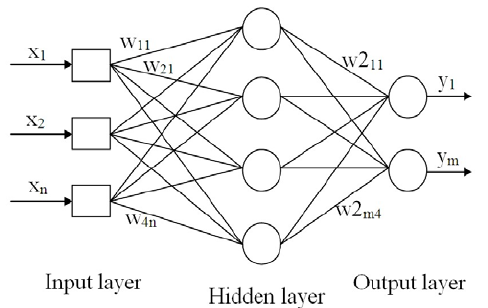
\includegraphics[width=.35\textwidth]{images/A-schematic-diagram-of-a-Multi-Layer-Perceptron-MLP-neural-network.png}
		\label{fig:mlayer-perceptron}}
	%\vfil
	\quad\quad
	\subfigure[from \citet{Deshpande2017}.]{
		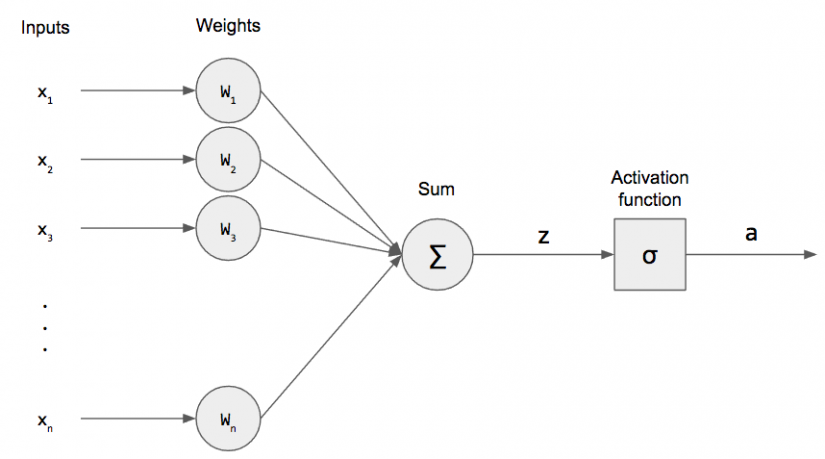
\includegraphics[width=.35\textwidth]{images/Single-Perceptron-825x459.png}
		\label{fig:single-perceptron}}
	\caption{(a) A multilayer perceptron comprised of layers of individual perceptrons. (b) An individual perceptron. TODO: reproduce myself}
	\label{fig:simple-ann}
\end{figure}
% directed acyclic graph, where nodes in the graph represent operations on data, and edges represent the flow of data through the graph. 
%This thesis will restrict itself to discussion of feedforward neural networks. 
%A feedforward neural network is an ANN where 
%Any recurrence will be unrolled to form a feedforward network. A feedforward 

\par
The set of parameters $\vtheta$ is usually learned, or trained, by stochastic gradient descent \citep{Bottou2011}.
Consider an ANN producing an approximated output $\hat{\vy} = f(\vx; \vtheta)$ and a cost function $J(\vy, \hat{\vy}) = J(\vy, \vx, \vtheta)$, with  $J$ being a differentiable function of its inputs, $\vy$ being the correct output of $f^*$, and $\vtheta$ being randomly initialized.
The cost function produces a scalar describing the error between $\vy$ and $\hat{\vy}$.
A common example of this is sum squared error, where $J(\vy, \hat{\vy}) = \sum_{n=o}^{i}(|\vy_n - \hat{\vy}_n|^2)$.
The gradient of $J$ with respect to the parameters is given by $\nabla_{\vtheta}J(\vy, \vx, \vtheta)$ and indicates the direction in which to move $\vtheta$ in order to increase $J$.
By iteratively applying $\vtheta = \vtheta - \epsilon \nabla_{\vtheta}J(\vy, \vx, \vtheta)$ (where $\epsilon$ is a scalar constant referred to as the learning rate), the value of $\vtheta$ will be modified such that $J(\vy, \vx, \vtheta)$ is minimized - thus maximizing the approximation accuracy of $f$.
$\vx$ and $\vy$ must be a randomly selected pair from the training set in order for this training process to represent the whole training dataset.
Whether this minimization lands on a global or local minimum is dependant on the function $J$.
\par


\section{Problem formation and scope}
\label{scope}
The aim of this thesis is to build upon existing research and develop a load forecasting system which can predict future load based on weather, holiday periods, car movement, and other factors. 
Bruny Island and the NAC will be used as a case study. 
The forecasting system is expected to be equally applicable to any power system network.
\\
Specifically, the system will have the following properties:
\begin{itemize}
	\item The system will produce a forecast up to 24 hours in the future in 15- to 60-minute intervals. This will be a rolling forecast that can be re-calculated at any time.
	\item The forecast will be able to begin from any point time.
	\item The forecast will predict load in kVA at each interval.
	\item The forecast system will be aimed at predicting aggregate load at the feeder level. That is, between approximately 0.5 and 10MVA.
	\item The forecast system will be especially tuned to predict load during holiday periods.
\end{itemize}
